\documentclass{article}

\usepackage{tikz}
\usepackage{listings}
\usepackage{xcolor}
\usepackage[width=6in, height=8in]{geometry}

\definecolor{codegreen}{rgb}{0,0.6,0}
\definecolor{codegray}{rgb}{0.5,0.5,0.5}
\definecolor{codepurple}{rgb}{0.58,0,0.82}
\definecolor{backcolour}{rgb}{0.95,0.95,0.92}
\definecolor{codeyellow}{RGB}{204,122,0}
\definecolor{codeblue}{RGB}{204,122,0}
\definecolor{codelightgreen}{RGB}{102,204,0}
\definecolor{codered}{RGB}{250,24,0}

\lstdefinestyle{mystyle}{
  rangeprefix=--\{\ ,
  rangesuffix=\ \}--,
  language=vhdl,                % choose the language of the code
  numbers=left,                   % where to put the line-numbers
  stepnumber=1,                   % the step between two line-numbers.        
  numbersep=5pt,                  % how far the line-numbers are from the code
  backgroundcolor=\color{white},  % choose the background color. You must add \usepackage{color}
  showspaces=false,               % show spaces adding particular underscores
  showstringspaces=false,         % underline spaces within strings
  showtabs=false,                 % show tabs within strings adding particular underscores
  tabsize=2,                      % sets default tabsize to 2 spaces
  captionpos=b,                   % sets the caption-position to bottom
  breaklines=true,                % sets automatic line breaking
  breakatwhitespace=true,         % sets if automatic breaks should only happen at whitespace
  title=\lstname,                 % show the filename of files included with \lstinputlisting;
  backgroundcolor=\color{backcolour},   
  commentstyle=\color{codegreen},
  keywordstyle=\color{magenta},
  numberstyle=\tiny\color{codegray},
  stringstyle=\color{codepurple},
  basicstyle=\ttfamily\footnotesize,
  breakatwhitespace=true,
  breaklines=true,                 
  captionpos=b,                    
  keepspaces=true,                 
  numbers=left,                    
  numbersep=5pt,                  
  showspaces=false,                
  showstringspaces=false,
  showtabs=false,                  
  tabsize=4,
  keywords={library,use,entity,component,port,generic,process,architecture,generate},
  alsoletter=<>\=-:&,
  comment=[l]{--},
  morekeywords={[2]&,=,<=,=>,:=,and,or,not,xnor,xor,mod,rem,true,false},
  keywordstyle={[2]\color{violet}},
  morekeywords={[3]rising_edge,signal,constant,attribute,variable},
  keywordstyle={[3]\color{teal}},
  morekeywords={[4]std_logic,std_logic_vector,boolean,integer,natural,bit,signed,unsigned,to_signed,to_unsigned,to_integer},
  keywordstyle={[4]\color{blue}},
  morekeywords={[5]begin,if,elsif,then,is,in,out,else,for,exit,loop,all,to,downto,others,report,until,with,select,until,case,end,of,transport,case,severity,when,wait,on,inout},
  keywordstyle={[5]\color{codeyellow}},
  morekeywords={[6]range,length},
  keywordstyle={[6]\color{codered}},
}

\lstset{style=mystyle}

\author{Tristan Itschner}
\title{VHDL Implementation of \\Direct Digital Synthesis}

\begin{document}

\maketitle

\tableofcontents

\section{Introduction}

% block diagram
\begin{figure}[ht]
\makebox[\textwidth][c]{
  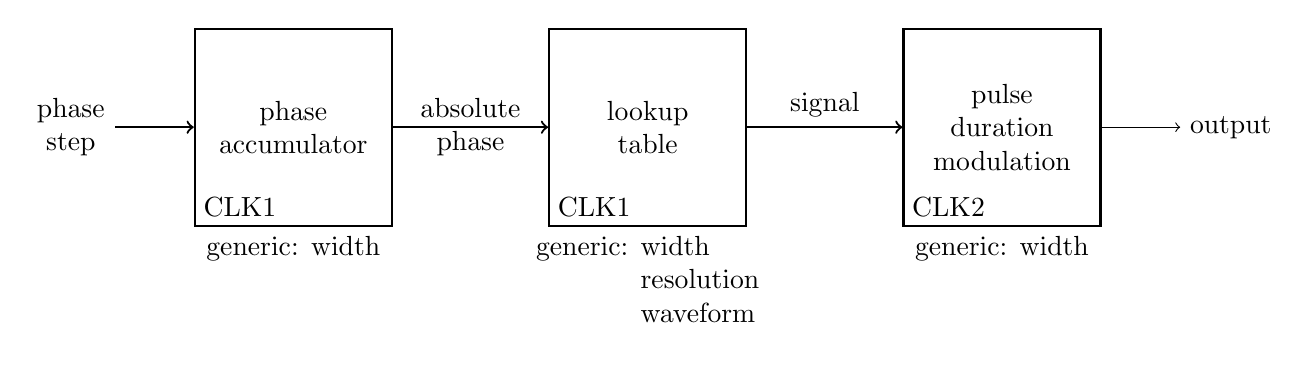
\begin{tikzpicture}
    \def\size{2.5cm}
    \def\sep{3.5cm}
    \node[align=center, rectangle, thick, draw, inner sep=0pt, minimum size=\size] (pa) {phase\\accumulator};
    \draw (pa.south) node[below] {generic: width};
    \node[align=center, rectangle, thick, draw, inner sep=0pt, minimum size=\size, right of=pa, xshift=\sep] (table) {lookup\\table};
    \draw (table.south) node[below, align=left] 
    {generic: width\\
    \phantom{generic: }resolution\\
    \phantom{generic: }waveform
  };
  \node[align=center, rectangle, thick, draw, inner sep=0pt, minimum size=\size, right of=table, xshift=\sep] (pdm) {pulse\\duration\\modulation};
    \draw (pdm.south) node[below] {generic: width};

    \draw[thick,<-] (pa.west) to ++(-1cm, 0) node[left,align=center] {phase\\step};
    \draw[thick,->] (pa.east) -- (table.west) node[midway, align=center] {absolute\\phase};
    \draw[thick,->] (table.east) -- (pdm.west) node[midway, above] {signal};
    \draw[->] (pdm.east) to ++(1cm, 0) node[right, align=center] {output};

    \draw (pa.south west) node[above right] {CLK1};
    \draw (table.south west) node[above right] {CLK1};
    \draw (pdm.south west) node[above right] {CLK2};
  \end{tikzpicture}
}
\label{main}
\caption{High-Level DDS Block Diagram (PL domain only)}
\end{figure}

Figure \ref{main} shows the high level diagram of Direct Digital Synthesis.

Direct Digital Synthesis (DDS) is a digital method of periodic signal
generation that has almost universally replaced prior analog methods.

\section{Components}

\subsection{Phase Accumulator}

The phase accumulator is nothing more than an adder, that continually adds the
input signal to its internal register, which is at the same time the output.

Common values of the registers width are 48 bits.

\lstinputlisting{../phase_acc.vhd}

\subsection{Lookup Table}

The lookup table converts the “time value” that is provided by the phase
accumulator into the corresponding signal value.

It is a block ram with usually one cycle of delay.

This block always runs at the same clock as the phase accumulator.

Usually only the MSbs of the input signal are relevant. This is due to the cost
of a large block ram. Still, the additional bits in the phase accumulator
provide better time resolution. They may also be used for interpolation
methods, to increase the signal resolution.

Common values are 16 bits, which is the likewise the limit for audio perception.

\lstinputlisting{../lookup_table.vhd}

\subsection{Pulse Duration Modulation}

Pulse Duration Modulation is a method of converting a digital signal into an
analog signal. It is similar to delta signal modulation (if not identical). The
PDM block is only one part, on the other end there must by an analogy
reconstruction filter.

The PDM utilizes a counter that is increased by one every cycle and has a width
that must be identical to the input signal resolution. The output signal is
merely 1 bit, and it is 1 if the signal value is above the counter value, else
it's 0. 

The PDM block may run at a faster frequency than the input signal. This allows
for a better signal reconstruction, as the edge frequency of the analog
recontruction filter may be choosen higher. Also a slower frequency on the
block ram side allows for a larger block ram.

\lstinputlisting{../pdm.vhd}

\subsection{DDS Wrapper}

\lstinputlisting{../dds.vhd}

\subsection{FAQ}

\begin{itemize}
  \item Why is the phase accumulator's register width greater than the lookup table?
\end{itemize}

\section{Testbench}

\end{document}
